\documentclass[10pt]{article}

% Adjust page margins if needed
\usepackage[margin=1in]{geometry}
 \usepackage{tabularray}
% Include necessary packages
\usepackage{setspace}
\usepackage{titlesec}
\usepackage{xspace}
\usepackage{array}
\usepackage{multirow}
 \usepackage{rotating}
\usepackage{tabularx}
% Set font to Times New Roman
\usepackage{mathptmx}
\usepackage{paralist}
\usepackage{graphicx}
\usepackage{subcaption}
\usepackage{float}
\usepackage{xcolor}
\usepackage{pifont}

\usepackage[T1]{fontenc}


\newcommand{\adaptdroid}{\texttt{AdaptDroid}\@\xspace}
\newcommand{\adaptdroida}{\texttt{AdaptDroid}\_a\@\xspace}
\newcommand{\android}{{\texttt{Android}}\@\xspace}
\newcommand{\appium}{\texttt{Appium}\@\xspace}
\newcommand{\architecture}{\texttt{Architecture}\@\xspace}
\newcommand{\atm}{\texttt{ATM}\@\xspace}
\newcommand{\atma}{\texttt{ATM}\_a\@\xspace}
\newcommand{\atmd}{\texttt{ATM}\_d\@\xspace}
\newcommand{\bert}{\texttt{BERT}\@\xspace}

\newcommand{\blogs}{\texttt{Blogs}\@\xspace}
\newcommand{\categories}{\texttt{categories}\@\xspace}
\newcommand{\corpus}{{\texttt{Corpus of Documents}}\@\xspace}
\newcommand{\craftdroid}{\texttt{CraftDroid}\@\xspace}
\newcommand{\craftdroida}{\texttt{CraftDroid}\_a\@\xspace}
\newcommand{\craftdroidd}{\texttt{CraftDroid}\_d\@\xspace}
\newcommand{\ES}{{\tt Edit Distance Similarity}\@\xspace}
\newcommand{\ede}{{\texttt{Event Descriptor Extractor}}\@\xspace}
\newcommand{\edes}{{\tt Event Descriptor Extractors}\@\xspace}
\newcommand{\selector}{{\tt Event Selector}\@\xspace}
\newcommand{\execplugin}{{\tt Executor-Plugin}\@\xspace}
\newcommand{\fscore}{\texttt{F1-Score}\@\xspace}
\newcommand{\fast}{\texttt{FastText}\@\xspace}
\newcommand{\plugin}{{\tt Fidelity plug-in}\@\xspace}
\newcommand{\fruiter}{\texttt{F}r\texttt{UIT}e\texttt{R}\@\xspace}
\newcommand{\glove}{\texttt{GloVe}\@\xspace}
\newcommand{\gp}{\texttt{Google-Play}\@\xspace}
\newcommand{\gt}{$e^t_{gt}$\@\xspace}
\newcommand{\project}{\texttt{HINTER}\@\xspace}
\newcommand{\projectfullname}{Highly Intelligent Test Reuse\@\xspace}
\newcommand{\imagelabeler}{\texttt{Image Labeler}\@\xspace}
\newcommand{\JS}{{\tt Jaccard Similarity}\@\xspace}
\newcommand{\manuals}{\texttt{Manuals}\@\xspace}
\newcommand{\mrr}{\texttt{MRR}\@\xspace}
\newcommand{\addrReproduction}{\href{https://star.inf.usi.ch/\#/software-data/11}{https://star.inf.usi.ch/\#/software-data/11}\@\xspace}
\newcommand{\matcher}{{\tt Semantic Matcher}\@\xspace}
\newcommand{\matchers}{{\tt Semantic Matchers}\@\xspace}
\newcommand{\patternbased}{{\texttt{Pattern-based}}\@\xspace}
\newcommand{\sma}{{\texttt{Semantic Matching Algorithm}}\@\xspace}
\newcommand{\smas}{{\texttt{Semantic Matching Algorithms}}\@\xspace}
\newcommand{\smcomponents}{{semantic matching components}\@\xspace}
\newcommand{\smconfig}{{\tt semantic matching configuration}\@\xspace}
\newcommand{\smconfigs}{{\tt semantic matching configurations}\@\xspace}
\newcommand{\sme}{{\tt Semantic Matching Evaluator}\@\xspace}
\newcommand{\tool}{\texttt{SemFinder}\@\xspace}
\newcommand{\topics}{\texttt{Topics}\@\xspace}
\newcommand{\toolreuse}{\texttt{EliteDroid}\@\xspace}
\newcommand{\tam}{{\tt Target Application Model}\@\xspace}
\newcommand{\generator}{{\texttt{Test Generator}}\@\xspace}
\newcommand{\generators}{{\tt Test Generators}\@\xspace}
\newcommand{\tme}{{\tt Test Migration Evaluator}\@\xspace}
\newcommand{\testreuse}{{\texttt{Test Reuse}}\@\xspace}
\newcommand{\topone}{\texttt{Top1}\@\xspace}
\newcommand{\use}{\texttt{USE}\@\xspace}
\newcommand{\wm}{{\texttt{WM}}\@\xspace}
\newcommand{\we}{{\texttt{Word Embedding}}\@\xspace}
\newcommand{\wem}{{\tt Word Embedding Model}\@\xspace}
\newcommand{\wv}{\texttt{Word2vec}\@\xspace}


\newcommand{\nevents}{8,099\@\xspace} %number of GUI event in isolation experiment
\newcommand{\ncomb}{337\@\xspace} %number of configurations in isolation
\newcommand{\ncombdomain}{240\@\xspace} %number of configurations for domain specific
\newcommand{\ncombtopic}{48\@\xspace} %number of configurations for domain specific
\newcommand{\ncombbasline}{192\@\xspace} %number of configurations for domain specific


%%

\newcommand{\nsampledcomb}{68\@\xspace} %number of sampled configurations
\newcommand{\nquery}{337\@\xspace} %number of queries
\newcommand{\ntotalscenarios}{248\@\xspace} %number of scenarios in ATM and CrafDroid paper
\newcommand{\ntotalapps}{42\@\xspace} %number of apps in ATM and CrafDroid paper [41 in ISSTA]
\newcommand{\nexescenarios}{147\@\xspace} %number of scenarios we could execute [139 in ISSTA]
\newcommand{\nexecapps}{30\@\xspace} %number of apps we could execute in isolation
\newcommand{\nreuseexecapps}{29\@\xspace} %number of apps we could execute in test reuse
\newcommand{\nbrokenapps}{12\@\xspace} %number of apps we could not execute
\newcommand{\nredundscenarios}{51\@\xspace} %number of redundant scenarios 
\newcommand{\nuniquecenarios}{95\@\xspace} %number of scenarios we used in isolation experiment
\newcommand{\nreusescenarios}{89\@\xspace} %number of scenarions we used in test reuse experiment
\newcommand{\nsharedscenarios}{27\@\xspace} %number of scenarions we used in test reuse experiment
\newcommand{\ntestcases}{34\@\xspace} %number of scenarions we used in test reuse experiment
\newcommand{\natmtestcases}{11\@\xspace} %number of scenarions we used in test reuse experiment
\newcommand{\ncrafttestcases}{23\@\xspace} %number of scenarions we used in test reuse experiment

\newcommand{\nmigrations}{6,000\@\xspace} %number of scenarions we used in test reuse experiment
\newcommand{\ninstances}{25\@\xspace} %number of scenarions we used in test reuse experiment


\newcommand{\ali}[1]{\textcolor{blue}{ \emph{\ding{46} Ali: #1}}}


% Title, author, and date
\title{\vspace{-3em} \project: \projectfullname}
\author{}
\date{}

\begin{document}

	\maketitle
	
		\section{Summary of the research plan}
	%1000 words
	% What should be included in here? summary of all below sections?
\ali{To be revised}

% What problem project aims to solve?
In this project we define a set of approaches to generate test cases for testing software applications through their Graphical User Interface. 
The generated test case are able to exercise the application under the test with realistic scenarios and reveal functional faults.


% What is the gap in the research?
Testing software applications is crucial to increase quality of a software. 
GUI testing tests software application at integration level to ensure its compliance to the functional requirements. 
Usually developers write test cases manually, which is tedious task and bears substantial cost on organizations.
Researcher have proposed many approaches to automate generating GUI test cases. 
Most of these approaches only are able to maximize code coverage and reveal faults that lead to system crashes.
Recently, researcher have proposed approaches that are aware of  semantics of applications and  test  intended functionality of the applications.


\testreuse is a promising category of automated GUI testing testing approaches that migrates tests of an application to another application with similar functionalities. 
These approaches are far from prefect, which hinders their applicability in industrial environment.
The current \testreuse approaches only rely on limited amount of information in the GUI to infer semantics and that leads to imprecise test migration with high uncertainty.


% What are the objectives? We do X to Y
In this project, we will address current limitations of \testreuse approaches by
\begin{inparaenum}[(i)]
\item using visual information of GUI to incorporate internal information in test migrations
\item using pattern of GUI interaction and web information to incorporate external information
\item defining strategies to build comprehensive model of target application GUI that facilitates navigation of \testreuse approaches in the target applications
\end{inparaenum}.

% How we do that? We use technique W to do X

We will leverage Artificial Intelligence to define set of \testreuse approaches and integrate them together to create a \textbf{H}ighly \textbf{In}telligent \textbf{Te}st \textbf{R}euse (\project) approach.
we will
\begin{inparaenum}[(i)]
\item incorporate Image Processing to extract visual information in the GUI
\item use Large Language Models to integrate their vast knowledge and pattern recognition capabilities into \testreuse
\item Reinforcement Learning  to efficiently build a model of target application GUI
\end{inparaenum}.
% How we validate the approach?
We will validate our approach on most popular applications from different domains of functionality to demonstrate it general applicability and it maturity to be used by practitioners.   


% What is the impact of the project?

This project will impact both research and industry. 
It will impact research in software engineering with approaches to generate realistic test cases at integration level, methodologies that can be reused in other areas such as test repair.
It will impact on development of software applications by with an approach that reveals functional fault, reducing cost of production and increasing quality of software. 










	\section{Research project}
	\subsection{Current state of research in the field }

\subsubsection{Terminology}

%%% Background knowledge
% What is GUI test case
% What is current state
% What is GUI model
\ali{to be revised}

A Graphical User Interface is a  forest hierarchical windows that only one of them at a time is active to be used.  
Windows includes atomic element named widget that are characterize by attribute, such as text or locations.
At any time the active window has a sate that encompasses attribute values of all visible widgets.
Type of widget depends on their functionality and some of them expose user-actionable events for users to interact with the application.

A GUI event is an atomic humane-computer interaction, such as click on a widget with the type button or fill an editable widget.
An oracle event check the state of a widget. 
For example, if a widget displays a specific text. 
A GUI test is a sequence of events $\langle e_1,..., e_n\rangle$ on widgets of active windows.
A test execution results transitioning the state of the active windows $S_{0} \xrightarrow{e_1} S_1 \xrightarrow{e_2} S_2 \ldots \xrightarrow{e_n} S_{n}$ 
%\), 
where $S_{i-1}$ and $S_i$ denote the states of the active window before and after the execution of $e_i$, respectively. 
A GUI model (\tam) is a directed graph where node correspond to GUI states  and edges correspond to events that transition the the source node (state before event) to the target node (state after the event).
% Test Reuse
% Semantic matching is one-to-one and using GUI model alleviate this issue.
% What is stepping events

\testreuse is the process of migrating test cases across apps with similar functionalities. 
\testreuse relies on semantic matching to find a corresponding event from the source test case in the target applications (one-to-one matching). 
Semantic matching uses textual attributes of widgets to score similarity of events.
The target test case may include stepping events, that are event not corresponding to any event in source test case.
The stepping event are required to reach relevant states.
The source test case may include  unmatchable events, that are event not corresponding to any event in target test case.
\testreuse handles stepping and unmatchable by relying on \tam.




\subsubsection{State of the art}
GUI testing has been a popular field in software engineering and 
researchers proposed many approaches that we classify into four categories: 
\begin{inparaenum}[(i)]
\item Random-based approaches take random actions to interact with the GUI~\cite{machiry:dynodroid:FSE:2013,ermuth:monkey:ISSTA:2016}.
\item Model-based approaches build a GUI model and generate test cases that cover the model based on coverage criteria~\cite{Gu:PractivalTest:ICSE:2019,Choi:swift:OOPSLA:2013}, 
\item Coverage-based approaches employ search-based algorithms~\cite{dong:TimaMachine:ICSE:2020} or symbolic execution to generate test cases that maximize code coverage~\cite{cheng:guicat:ASE:2016},
\item Semantic similarity-based approaches use existing knowledge of testing functionalities of applications to generate test cases for applications with similar functionalities.
%All the categories except for similarity-based are agnostic to the semantics of the application under the test. 
Non-semantic approaches quickly generate many test cases with high coverage, but they only reveal crashing faults and cannot expose functional faults.
\end{inparaenum}
% Pattern-

\smallskip 
Millions of applications share similar functionalities that create an opportunity to test them similarly.
For example, online booking of flights can be tested similarly across different applications. 
Similarity-based approaches leverage this opportunity and generate test cases relevant to the functionality of the applications.
We classify similarity-based approaches into pattern-based and \testreuse.
Pattern-based approaches consider patterns comprising abstract recurrent events and match elements of the pattern to actual events in the target application~\cite{mao:crowd:ASE:2017,Mariani:Augusto:ICSE:2018}.
%~\cite{Moreira:pattern:ISSRE:2013,Morgado:Impact:HCI:2019}.
%They either consider a predefined set of patterns~\cite{Mariani:Augusto:ICSE:2018,Hu:appflow:FSE:2018} or automatically extract patterns from traces of user interactions~\cite{mao:crowd:ASE:2017,Mao:UserPattern:JSS:2021}.
Crafting patterns manually requires substantial human effort, while extracting patterns automatically requires enormous data.


\smallskip 
\testreuse approaches leverage semantic similarity of textual information available in the GUI to migrate test cases across applications.
Researchers proposed approaches that migrate test cases of the same application across different platforms~\cite{talebipour:MAPIT:ASE:2021} and different applications in the same platform\cite{rau:efficent:icse:2018}. 
%TestMig migrates test cases from the IOS version of an app to its Android version~\cite{Qin:testmig:ISSTA:2019}.
%MAPIT migrates test cases bidirectionally between IOS and Android versions of the same app~\cite{talebipour:MAPIT:ASE:2021}.
%TransDroid migrates test cases of web apps to their Android version~\cite{lin:TransDroid:ICST:2022}.
% Rau et al. proposed migrating test cases in web applications  using semantic matching of GUI elements~\cite{rau:efficent:icse:2018}.
In this project, we focus on the latter type since they have a broader applicability.
 \craftdroid~\cite{lin:craftdroid:ASE:2019} and \atm~\cite{Behrang:migration:ICSE:2018} migrates test cases across Android apps.
%GUITestMigrator migrates test cases between prototype apps that share the same specifications.
%\atm is an extension of GUITestMigrator that migrates test cases of real apps~\cite{Behrang:migration:ICSE:2018}.
 \adaptdroid formulates \testreuse as a search problem and uses an evolutionary algorithm to explore the space of possible GUI test cases~\cite{Mariani:Adaptdroid:AST:2021}.
 
 
\smallskip 
Researchers exploited Machine Learning techniques to propose enhanced approaches in different categories of GUI test generation.
%Vision
APPFLOW uses computer vision to match elements of predefined patterns to the GUI elements of the target application~\cite{Hu:appflow:FSE:2018}.
%AVGUST leverages computer vision to extract patterns from screen recordings of users interacting with apps~\cite{zhao:Avgust:FSE:2022}.
White et al. proposed a random approach that detects the type of widgets from their visual appearance~\cite{white:WidgetDetection:ISSTA:2019}.
%%%%Their approach determines the widget type, such as the menu or text box. However, it does not provide information about the semantics of widgets.
%Zhu et al. proposed an approach for identifying the intent of widgets~\cite{zhu2021widgetrecog}.
%%%%However, their approach is not examined in the GUI testing context. 
% RL
%%%%%%%%
DeepGUI uses deep reinforcement learning (RL) and computer vision to identify and select actionable events~\cite{YazdaniBanafsheDaragh:DEEPGUI:ASE:2021}.
Some approaches used reinforcement learning to model the behavior of the GUI and select events.
A-test~\cite{Vuong:RLTest:A-Test:2018} use Q-Learning to generates test cases  for Andoroid apps.
%ARES uses deep learning to infer state similarities, while previous approaches used tabular reinforcement learning~\cite{Romdhana:ARES:TOSEM:2022}.
Recently, researchers used Large Language Models (LLM) to generate inputs for editable widgets in random GUI testing ~\cite{liu:GUIInputLLM:ICSE:2023} and to transform natural language commands into GUI test cases~\cite{Zimmermann:GPT3GUITest:2023:ICSTW}. 

% limitations of current test reuse approaches

\smallskip 
%\testreuse approaches are the most recent category of GUI test generations, which can expose functional faults by exercising realistic scenarios. 
Our review of the state of the art and our empirical studies of \testreuse~\cite{mariani:SemFinder:ISSTA:2021,khalili:DomainEmbedding:ICPC:2022} suggest we can address the limitations of current \testreuse approaches by using advanced machine learning techniques. 
The first limitation is that the current \testreuse approaches ignore visual information, and they only rely on text, which may not be sufficient. 
In this project, we will leverage computer vision to address this limitation by combining visual and textual information.
Additionally, we will use LLM models to incorporate web information that is integrated into their train set to improve \testreuse. 
The second limitation is that current approaches explore the target application by relying on \tam, which is often incomplete.
In contrast to model-based approaches that replaced the \tam with an RL agent, we will use RL to create a more comprehensive model.


\subsubsection{Current Research Projects}

%Software testing is an important topic that is the subject of many research projects. 
The applicant is aware of the following relevant research projects:
 \textit{Self-assessment Oracles for Anticipatory Testing} (P.I. Paolo Tonella) focuses on the problem of testing machine learning, while \project uses machine learning to test GUI applications. \textit{A-Test Autonomic Testing} (P.I. Mauro Pezze) focuses on testing distributed systems in the production environment and uses machine learning for different types of applications and environments from this project. The first two projects are funded by ERC, and the last project is funded by SNF. 




		
\subsection{Current state of own research and professional competences for the project}
\label{sec:own-research}
% 1000 words

\begin{figure}[h]
	\centering
	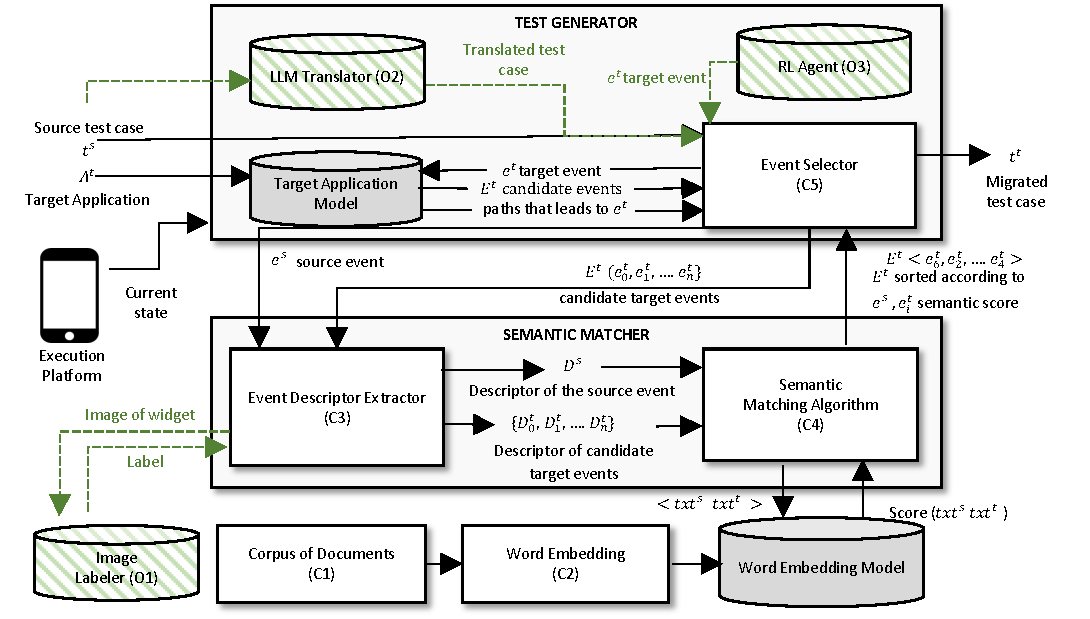
\includegraphics[width=\textwidth]{images/architecture.pdf}
	\caption{\testreuse architecture and project objectives}
	\label{fig:architecture}
\end{figure}

%Test Reuse architecture
We reviewed state-of-the-art \testreuse approaches for Android, \atm~\cite{behrang:apptestmigrator:ASE:2019}, \craftdroid~\cite{lin:craftdroid:ASE:2019}, and \adaptdroid~\cite{Mariani:Adaptdroid:AST:2021} by full replication of their experiments, and careful inspection of their source code that is publicly available.
We proposed a general \architecture for \testreuse based on our review that abstracts common components of \testreuse approaches and their interactions. 
The \architecture enables us to study \testreuse approaches in more depth, and guide researchers in developing new approaches.
C1, C2, C3, C4, and C5 are the components that we identified in the current approaches and O1, O2, and O3 (in hashed green) are the realization of \project objectives that we explain in section \ref{sec:detailed-plan}. 


% Test Ruse work flow
\smallskip 
\testreuse  includes two coarse grain parts: \generator and \matcher, which collaborate to migrate source test case $t^s$ to target test case $t^t$.
\generator receives the $t^s$ and selects a match for each source event $e^s \in t^s$ in the target application $A^t$.
For each $e^s$, the \generator considers a set of target candidate event $E^t$ from the \tam and the current GUI state. 
Then, it queries the \matcher to sort the candidates based on their similarity to the $e^s$.
\generator selects an event from the sorted candidates and executes the event, transforming the current GUI state to another. 
After iterating over all the $e^s \in t^s$, the selected target events from $A^t$ comprise the migrated test case.



\smallskip 
In more detail, the \generator statically analyzes $A^t$ to create a \tam and updates the model as it progresses in migrating $t^s$.
The \selector gathers a set of target candidate events $E^t$ for each event $e^s$ and selects from the candidates, which are sorted by \matcher.
If the \selector selects an event from the current GUI state, it executes the event and adds the event to the migrated test case.
If the \selector selects an event from the \tam, the event is absent in the current state and the \selector queries the \tam to find a path to the state where the selected event exists.
Then, it executes the selected events (including the stepping events) and adds them to the set of migrate test cases.
If the \selector does not select any event from $E^t$, it will skip the $e^s$.
\testreuse approaches implement the \selector strategy differently.


\smallskip 
The \matcher receives a query containing the $e^s$ and $E^t$, then the \ede (C3) extracts descriptors of events $D$.
A descriptor consists of textual attributes associated with the widget of an event such as \textit{resource-id}.
For each pair of $\langle D^s,  ~D_i^t\rangle$, the \sma queries the \wem to score similarity of their textual attribute, then it aggregates the scores to sort the $E^t$.
The \wem encodes words (or sentences) to vectors, representing the semantic distance of the words.
The \wem is built by one-time training of a \we techniques(C2) on a given \corpus (C1). 
Components of \testreuse can be implemented in different ways, and we call the implementation an instance of the component.
Each combination of instances of the \matcher components (C1-C4) yields a unique \smconfig that answers the semantic matching queries differently.
 Figure~\ref{fig:architecture} shows four out of five \testreuse components are located in \matcher, which emphasizes on crucial role of semantic matching.
 This observation motivated us to in-depth study semantic matching, identify its limitations, and propose new solutions. 

\smallskip 
 First, we studied semantic matching in isolation from \testreuse to eliminate the side effects of other \testreuse parts~\cite{mariani:SemFinder:ISSTA:2021}.
In our study, we created different \smconfigs to answer  a set of queries and we evaluated their performance to measure the effectiveness of instances and the impact of components.
We considered instances from the literature, and we introduced a new instance for the \sma named \tool and a new \corpus named \gp that we collected from crawling around 1 million apps in Google Play. 
In total, we considered \ninstances instances that resulted in \ncomb configurations.
We used the configurations to answer \nquery queries that we extracted from experiments of \testreuse approaches.
We evaluated the configurations using standard metrics such as \mrr~\cite{liu:MRR:learning:2009} that measure how many correct matches  appear on the top positions in the sorted list of target candidates on average. 
The results showed the most impactful component is the \sma, followed by \we, \ede, and \corpus. 
Also, our newly proposed instances outperformed the existing ones. 



\smallskip 
Second, in the study of semantic matching in isolation, we observed our newly proposed corpus \gp, which is specific to the mobile applications domain, leads to better results than general corpora.  
However, the impact of the \corpus component was the lowest, indicating the instances of this component perform closely. 
We hypothesize further specialization of the \corpus  potentially leads to better semantic matching.  
Thus, we used topic modeling to create domain-specific word embedding models, and then we investigated models  impact on semantic matching.
Our results showed that domain-specific models generally work better, but too much specialization deteriorates the performance~\cite{khalili:DomainEmbedding:ICPC:2022}.



\smallskip 
Third, we studied semantic matching in the \testreuse context (EMSE In Press).
We built a framework named \tme that automatically migrates test cases with different \smconfigs and evaluates the test cases based on the fidelity metrics that have been proposed in the literature~\cite{zhao:fruiter:fse:2020}.
In a nutshell, we used an \fscore metric that indicates how much the generated test case matches the source test case with respect to the ground truth.
In our experiment, we considered  \nexecapps apps from \atm and \craftdroid studies.
We excluded \adaptdroid~\selector because it is computationally too expensive, and it would have drastically limited the scale of our experiment.
In addition, migration of the test cases in our data set with all the \smconfigs takes more than 1000 days of computation, thus we sampled the configurations to select an affordable wide range of configurations.  
We selected \nsampledcomb configurations and performed more than \nmigrations migrations.
The results showed a strong to medium correlation between semantic matching and \testreuse, following the classification of Cohen~\cite{cohen:statisticalpower:Routledge:2013}.
In our study, we  thoroughly discussed the impact of components, the effectiveness of instances, and how they can be affected by different setups such as choice of \selector and subject apps.

\smallskip 
Figure~\ref{fig:MRR-F1-scatter} shows a part of our results that is related to the correlation of semantic matching and \testreuse.
The red triangle indicates a random baseline configuration that randomly scores the similarity of events.
The green square indicates an artificial perfect semantic matching that we synthesized based on the ground truth, and it  assigns a score of 1 to the correct match and 0 otherwise.
The blue dots indicate the sample configurations.
The figure shows a considerable gap between the current \smconfigs and the perfect configuration. 
Our manual inspection suggests ineffectiveness of semantic matching is due to the lack of textual information in the events descriptors.
The figure also shows even the perfect matching does not lead to a perfect \testreuse (\fscore of one).
The reason is that in some conditions, the \tam is not complete enough to find a matching event in a state other than the current one or a path to the matching event.




\begin{figure}[H]
	\centering
	\begin{subfigure}{.5\textwidth}
		\centering
		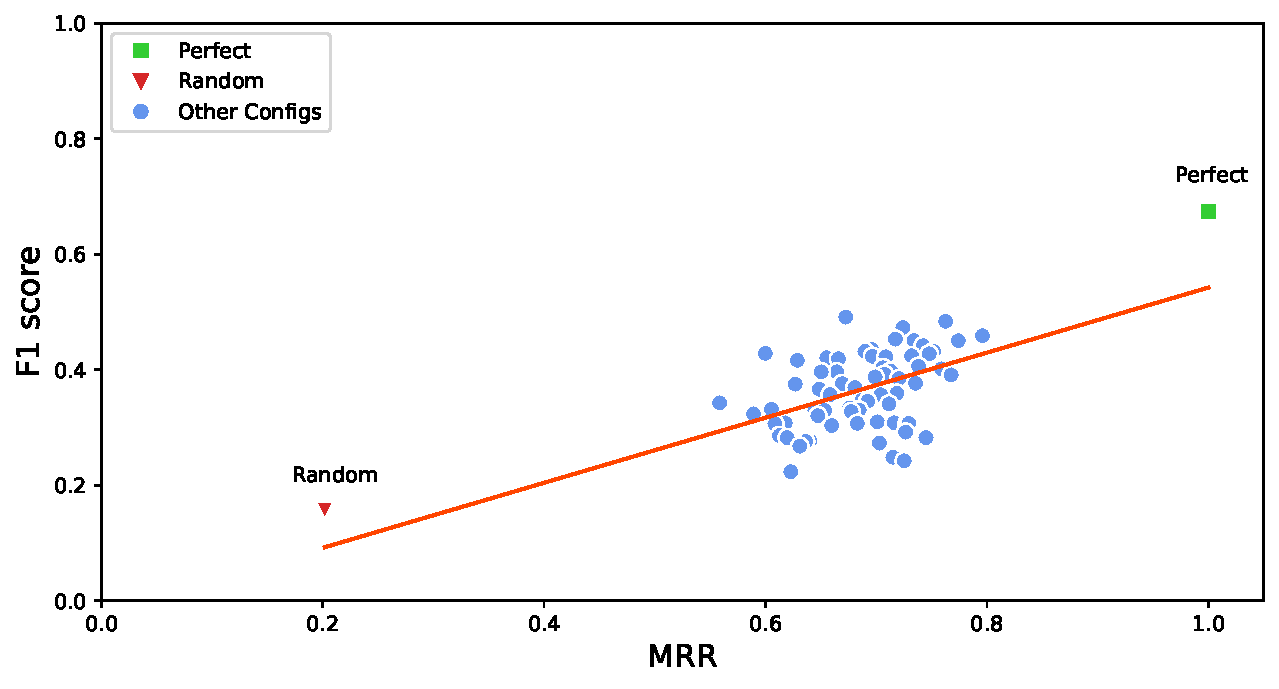
\includegraphics[width=1\linewidth]{images/MRR_craftdroid_all_oracle_included.pdf}
		\caption{\craftdroid as selector}
		\label{fig:MRR_craftdroid_all_oracle_full}
	\end{subfigure}%
	\begin{subfigure}{.5\textwidth}
		\centering
		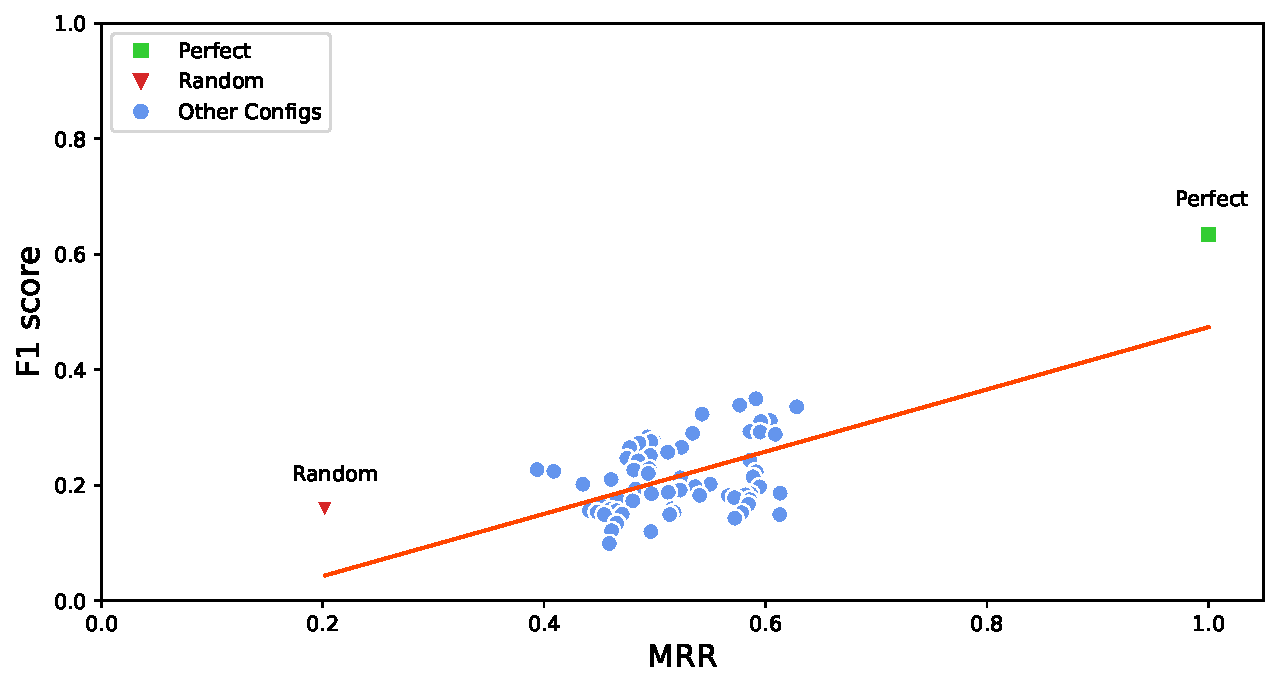
\includegraphics[width=1\linewidth]{images/MRR_atm_atm_oracle_included_passfree.pdf}
		\caption{ ATM as selector}
		\label{fig:MRR_atm_atm_oracle_passfree_full.pdf}
	\end{subfigure}
	\caption{Correlation between semantic matching (\mrr) and \testreuse (\fscore)}
	\label{fig:MRR-F1-scatter}
\end{figure}

\ali{to be revised}

\noindent
\textbf{Professional Competence:}

\noindent
The applicant gained research competence the subject of this project, \testreuse, in his PhD studies.
The applicant has obtained the relevant IT skills and knowledge in relevant areas during his undergraduate and graduate studies in software engineering.
















	\subsection{Detailed research plan}
% 2000 words

%In the previous section we explained the two identified challenges of \testreuse:
In section~\ref{sec:own-research} we described the two challenges of \testreuse that we identified in our studies:
%lack of information in the GUI and uncertainty of \testreuse when semantic matching is not helpful.
Lack of textual information in the GUI, and uncertainty of current semantic matching approaches in absent of one-to-one mapping. 
%In this section we explain how objectives of the project will address these challenges. 
In this section we elaborate what are the objectives of \project project and how they address the two challenges.

\bigskip
\noindent
\textbf{O1:} to augment semantic matching with internal information other than text.  
We will use computer vision to incorporate visual information of GUI in the semantic matching.  

\bigskip
We will overcome the first challenge by using both textual and visual information available in the GUI.
In fact, users interact with apps by relying on both textual and visual information in the GUI to navigate through app windows and execute their intended functionalities. 
Additionally, most apps consider UI design best practices which emphasis on compliance of UI with users prior knowledge.  
 Thus, users expect elements with same visual cues provide similar functionalities across different applications.
For example, users expect text box with a nearby magnifier icon  provide the search functionality.
Current semantic matching approaches for \testreuse are agnostic to visual cues, while both user and developer rely on these cues to communicate possible functionalities in the app. 


%%% Maybe I need to move it to related works
\bigskip
Researchers used computer vision in many software engineering areas such as test repair~\cite{Stocco:VisualRepair:FSE:2018,Pan:Meter:TSE:2022,Xu:GUIDER:ISSTA:2021}  test generation~\cite{YazdaniBanafsheDaragh:DEEPGUI:ASE:2021,Li:Humanoid:ASE:2019,Hu:appflow:FSE:2018}, and widget recognition~\cite{zhu2021widgetrecog, white:WidgetDetection:ISSTA:2019}.
White et al. proposed an approach to improve random GUI testing by widget detection~\cite{white:WidgetDetection:ISSTA:2019}. 
%However, their approach only determines type of the widget and not its semantic.
Their approach determines the widget type like menu or text box, however, it does not provide information about semantics of widgets.
%Zhu et al. proposed an approach for identifying intent of widget and labeling them. 
Zhu et al. proposed an approach for identifying the intent of widgets and labeling them to describes the widget function~\cite{zhu2021widgetrecog}. 
However, their approach is not examined in GUI testing context. 

%%% Edite from here !!!!

\bigskip
We will create a module named \imagelabeler encompassing the encode-decoder architecture to transforms widget images to the textual description of their functionality.
We will integrate the \imagelabeler to the \testreuse~\architecture  as depicted in figure~\ref{fig:architecture} to enhance the semantic matching.
The \ede  will uses widgets coordination available in the DOM to crop images of widgets form the screenshot of the GUI.
Then, \ede queries \imagelabeler to get description of  widget images.
\ede adds the image description as another attribute of event descriptor $D$ and \matcher proceed as before.


\bigskip
%Training or fine-tuning models to generate text usually requires large train set and expensive computational resources which could be out of scope of this study. 
Training or fine-tuning models for generating text requires large train set and expensive computational resources that could be out of scope of this study. 
%If we encounter this blocking risk, we can take an alternative approach that relies on classification of images.
If this risk occurs, we will use image classification as an alternative approach.
%Similar to \texttt{AppFlow} approach, we  will  classify GUI widgets to a canonical representation that we define in advance. 
We will define canonical representations of widget  (classes) in advance and build a classifier that assigns widget to the classes.
%We assign labels to the canonical widgets that we will use to enhance the semantic matching.
We will label the canonical widgets with description of their functionalities.
%For example, we assign "back" label to the icon with a left arrow and \imagelabeler sends "back" label  to \ede for any widget that classifier consider in this class.  
For example, we assign "back" label to the icon with a left arrow.
 When \ede queries \imagelabeler, first it classifies the widget, then it returns the label of the canonical widget.
%We will use both set of canonical widgets in the literature , and we will review a large set of popular applications to identify most common widgets that has not been considered in the literature.
We will consider available canonical widgets in the literature and identify the most common widgets that are missing in the literature. 

















\bigskip
\noindent
\textbf{O2:} to use external resources of information containing patterns of functionalities. We will use LLM to translate test cases before reuse.

\bigskip
When users interact a new applications they, consider two strategies: 
a) they use their prior knowledge of using applications with similar functionalities to navigate through the new application. 
b) They leverage patterns of interactions that they leaned  in using the new application. 
Additionally, they can search in the web to understand functionalities of an application. 
LLM models can imitate both strategies of users:
a) They can recognize sequence of interactions belongs to what pattern
b)  They contain knowledge about wide variety of topics including applications functionalities.

\bigskip
We will use LLM to add more information from external resources to mitigate lack of information in the GUI.
In a simple word LLM transforms the input text to human like text. 
We can formulate problem of reusing test cases as giving sequence of text that represents source test case and contextual information as input to LLM and receive a target test case as output.  
In the \testreuse scenario, textual context is information available in the GUI of target application. 
The LLM model recognize the interaction pattern that source test belongs to, (for example, sign-in) then generates a test case for the target application with respect to the contextual information.

\bigskip
Integrating LLM in the \testreuse process requires two steps: Prompt Generation and Fine-tuning. 
%
Each prompt includes a source test case, and the contextual information of the target application. 
We consider the textual information as set of available event in each windows.
%
In Fine-tuning, we create a set of prompts and their answers.
A prompt answers is a test case that is migrated by an expert. 
% 
The output may contain events that are unreachable immediately from the previous event and  some stepping events needs to be considered to become reachable.
 Thus, we use the transformed test case as input of a conventional GUI test reuse to validate and add the stepping events to the test case. 


%%% Risk
\bigskip
A possible risk is that the generated test cases contains many unreachable events that bears too much cost on the conventional \testreuse approaches.
An alternative way to address this risk is to consider deliberate prompt engineering and presenting the contextual information such that contain graph nature of the GUI as each window in the GUI (nodes) includes multiple possible events and each events transfers the current state to another window (edges).

\bigskip
\noindent
\textbf{O3:} to make \testreuse robust in present of uncertainty. We use Reinforcement Learning to guide test reuse in absent of a matching event.

\bigskip
In the cases that a matching event is unavailable in the current state, \testreuse approaches use the GUI model of the application to create stepping event and reach an state where the matching event is available. 
\testreuse approaches create the GUI model  by static analysis of the application and complete it as they go through the \testreuse process. 
But, the GUI model is often incomplete and events may remain unreachable. 
Other times semantic matching cannot find any matching event neither in the current state nor in the GUI model. 
In such conditions that semantic matching is ineffective, \atm and \adaptdroid consider a random action, however, that is not always helpful and may result in many false positives. 
We will use Reinforcement Learning in the \testreuse to handle the uncertain condition.

\bigskip
Training a Reinforcement Learning agent requires defining states, reward function, and actions.
We define the states as set of textual attributes of widget available in the GUI state and we consider the reward function the same as the reward function of AutoBlackBox~\cite{Mariani:Autoblacktest:ICSE:2011} which is  how much the new state is different in comparison to the previous states. 
%
We use Reinforcement Learning in two stages: 
First, we use RL to explore the GUI before start of \testreuse process. 
Since the reward functions values  novel states it the agent will explore GUI effectively and we can create a more comprehensive model of the GUI automatically. 
Second, in conditions that semantic matching is  ineffective, the \testreuse approach queries the agent for the next actions.
Our intuition is that the agent will transform the state to novel state that might contains an event match. 
We will limit number of consequent actions that agent takes to handle conditions that a matching event do not exist at all.



	
	\subsection{Schedule and milestones}
% 1000 words

% \usepackage{rotating}
% \usepackage{multirow}


\begin{table}[h!]
	\centering
	\caption{Research Plan}
	\label{tab:research-plan}
	\begin{tabular}{|m{1cm}|m{1cm}|p{4cm}|p{4cm}|p{4cm}|} 
		\cline{2-5}
		\multicolumn{1}{c|}{\multirow{2}{*}{}}                      & \multirow{2}{*}{\textbf{Duration}}     & \multicolumn{3}{c|}{\textbf{Objectives}}                                                                                                                                                                                                                                                                                                                                                                                                                                                                                                                                                                                                                                                                                                                                     \\ 
		\cline{3-5}
		\multicolumn{1}{c|}{}                                       &                                        & \textbf{O1 (Internal Resources)}                                                                                                                                                                                                                                                             & \textbf{O2 (External Resource)}                                                                                                                                                                                                               & \textbf{O3 (Robustness)}                                                                                                                                                                                                                  \\ 
		\hline
		\rotatebox{90}{\textbf{\textbf{Study}}}      & \rotatebox{90}{2 months} & Studying computer vision approaches for classifications of images             Choosing most suitable approach in context of test reuse                                                                                                                                           & Studying LLM approaches             Identifying suitable prompts template                                                                                                                                                                     & Studying RL approaches             Identifying suitable RL approaches in Test Reuse context             Identifying different options for representing states and rewards                                                                 \\ 
		\hline
		\begin{sideways}\textbf{\textbf{Experiments}}\end{sideways} & \begin{sideways}4 months\end{sideways} & Collecting trainset and training a vision-based classifier             Integrating CraftDroid with the classifier             Experimenting on Subjects used by our previous study for generating test cases             Experimenting on new Subjects for generating test cases & Preliminary experiments with different LLM approaches and prompts and choose the best one             Fine-tuning LLM models             Integrating CraftDroid with the LLM models             Experimenting on all of subjects that we have & Preliminary experiments with different representation of states             Using RL in present of uncertainty             Using RL to explore GUI and make GUI model complete             Experimenting on all of subjects that we have  \\ 
		\hline
		\begin{sideways}\textbf{\textbf{Report}}\end{sideways}      & \begin{sideways}2 months\end{sideways} & Submitting a workshop paper from the preliminary studies             Submitting a research conference paper                                                                                                                                                                                                          & Submitting a workshop paper from the preliminary studies             Submitting a research conference paper                                                                                                                                   & Submitting a journal paper                                                                                                             \\
		\hline
	\end{tabular}
\end{table}

Table~\ref{tab:research-plan} summarizes the schedule and milestones of the \project project.
We will achieve a milestone corresponding to an objective by completing three steps: Study, Experiment, and Report. 
 In the study phase, we will review the related works.
In the experiment phase, we will gather: a complete data set for training models, build a new \testreuse approach, and empirically evaluate the approach. 
In the report phase, we will submit the results of experimenting with our approaches in  the top research venues in Software Engineering.
%We explain the details of milestones below.

\smallskip
\noindent
\textbf{O1: Incorporating Internal Resources:}  

\noindent
In the study phase, we will review vision-based GUI testing~\cite{Hu:appflow:FSE:2018,zhao:Avgust:FSE:2022,YazdaniBanafsheDaragh:DEEPGUI:ASE:2021}  and widget recognition approaches~\cite{white:WidgetDetection:ISSTA:2019,zhu2021widgetrecog}. 
We will examine the replication package and data sets of these studies, and in case of compatibility with our context, we will reuse them. 
Otherwise, we will study image captioning and classification approaches to build our model for the \imagelabeler component.
%\bigskip
%There is a risk that existing approaches for recognition of widgets will not be replicable. 
%In that case we need to take an alternative route which is classifier type, building training set, and training a classifier.  
%Therefore, we study computer vision approaches to identify most suitable classifier. 
%The most common approach for image classification is Convolutional Neural Networks (CNN)~\cite{lecun1995convolutional}. 
%Using CNN requires careful choice of its architecture depending on the down stream tasks. 
%We will investigate the most popular choices that includes: ResNet~\cite{he:ResNet:CVPR:2016}, Inception~\cite{szegedy:inception:CVPR:2015}, MobileNet~\cite{howard:mobilenets:arxiv:2017}.
%
%\bigskip

\smallskip
We will transition from the study to the experiment phase by conducting a feasibility study. 
%We will investigate from suitable approaches that we identified which one is more promising in our context.
We will select the most promising technique for labeling  widgets that is suitable in our context.  
To do so, we will experiment with different prototypes of \imagelabeler for semantic matching in isolation from the \testreuse,  similar to our previous study~\cite{mariani:SemFinder:ISSTA:2021}. 
Then, we will integrate \imagelabeler in our \tme framework to create a new \testreuse approach named \visiontool\footnote{Horus is a god in ancient Egyptian mythology that symbolizes heightened vision.}.
Additionally, we will use our~\tme framework to evaluate \visiontool and compare with the state-of-the-art \testreuse approaches.

\smallskip
Finally, we will submit the results of our  feasibility study to a workshop conference and the result of the \testreuse experiments to a top software engineering conference. 

%%% O2


\smallskip
\noindent
\textbf{O2: Incorporating External Resources:}  

\noindent
In the study phase, we will review LLM-based GUI testing approaches~\cite{Zimmermann:GPT3GUITest:2023:ICSTW, liu:GUIInputLLM:ICSE:2023} and prompt engineering, as a recent study shows tuning prompts improve specialised tasks such as code summarization  by 26\% on average~\cite{wang:prompt:FSE:2023}.
%\bigskip

\smallskip
We will transition from the study phase to the experiment phase by conducting a feasibility study that examines different LLM models and prompt patterns.
%We will investigate the applicability of existing LLM models in our context and if they require fine-tuning.
We will examine different combinations of LLM models and prompt patterns to translate a limited number of test cases.
We will manually inspect their quality and choose the most promising combination.
After the feasibility study, we will integrate the \llmtranslator into our framework to create a new \testreuse approach named \llmtool\footnote{Hermes is a god in ancient Greek mythology that symbolizes linguistic prowess.}.
Additionally, we will use our \tme framework to evaluate \llmtool and compare with the state-of-the-art \testreuse approaches.

\smallskip
Finally, we will submit the results of our  feasibility study to a workshop conference and the result of the \testreuse experiments to a top software engineering conference. 


%%% O3


\smallskip
\noindent
\textbf{O3: Improving Robustness:}  

\noindent
%study
In the study phase, we will review Reinforcement Learning based  GUI testing approaches~\cite{Pan:QTesting:ISSTA:2020,Romdhana:ARES:TOSEM:2022}. 
We will identify suitable options for the RL techniques, state presentation, and reward function.
%Experiment

\smallskip
We will transition from the study to the experiment phase by  conducting a feasibility study, in which we evaluate the candidate \rlaganets performance based on the number of distinctive windows  explored in a given amount of time. 
After the feasibility study, we will  integrate the best \rlaganet in our framework to create a new \testreuse approach named \rltool\footnote{Athena is a goddess in ancient Greek mythology that symbolizes strategic intellect.
}.
\rltool subsumes \visiontool and \llmtool by  encompassing \imagelabeler and \llmtranslator components.
Additionally, we will use our \tme framework to evaluate \rltool and compare with the state-of-the-art \testreuse approaches.
%We will evaluate the effectiveness of \rlaganet in three setups:
%\begin{inparaenum}[a)]
%	\item The agent only executes before \testreuse to make GUI model more complete
%	\item The agent only executes when semantic matching is uncertain
%	\item The agent executes both in the beginning and uncertain conditions.
%\end{inparaenum}

\smallskip
Finally, we will submit the \rltool in a tool track of a conference and the result of the \testreuse experiments in a top software  engineering journal to conclude the project. 


















	\subsection{Relevance and impact of the research }


In the past decades, researchers focused on automated GUI testing as a suitable solution for reducing the cost of integration testing. However, the current solutions have not been wildly used by practitioners due to their limitations. 
Our approaches address the limitations and impact both research and industry as follows:


% on research 


\smallskip
\noindent
\textbf{Research:}

\noindent
This project produces mature \testreuse approaches, and it will impact the broader field of GUI testing by following contributions: 
\begin{inparaenum}[(i)]
\item proposes a set of prompt patterns that formulates \testreuse as a prompt answering problem 
\item proposes strategies for building comprehensive  \tam
\item enhances the effectiveness of semantic matching techniques.
\end{inparaenum}

\smallskip
The first two contributions impact model-based approaches from two aspects.
First, integration of GUI model in prompts opens a new direction to use LLM for model-based testing.
Second, a comprehensive model improves coverage of the  generated test cases.
Effective semantic matching influnce Test Repair and Pattern-based approaches, both of which rely on semantic matching.
Test repair approaches find replacements for events that are broken in a test case between two versions of an app by matching the broken event to a semantically equivalent event in the new version~\cite{Pan:Meter:TSE:2022}.
Pattern-based approaches use semantic matching to match elements of an abstract pattern to events of the target app.


\smallskip
\noindent
\textbf{Industry:}

\noindent
The approaches that we introduce in this project are applicable to all types of applications that include GUI interactions, such as E-commerce and mobile apps.
E-commerce sales exceeded 6 trillion U.S. dollars worldwide~\footnote{\href{https://www.statista.com/topics/871/online-shopping/}{E-commerce worldwide - statistics \& facts}} in 2023.
%These commercial sectors are just a subset of industries that depend on GUI applications, and the financial cost of software failure is substantial in them.
The financial cost of software failure is substantial in these sectors.
In this project, we will create a standalone tool, \rltool, that developers can use to reveal functional faults, improve software quality, and ultimately increase business revenues.
%
Additionally, we will introduce an effective semantic matching technique that is applicable not only in testing but also in business logic.
Many organizations analyze available data on the web to make business decisions or provide insights. 
Various sources may represent the same data differently, which decreases analysis accuracy. 
Developers can leverage semantic matching approaches to overcome this issue.

	
	\subsection{Relevance for personal career development }
%750 words

%The milestones and the objectives are designed  mutually exclusive to create oppurtunity of parallization. 
%In case of collaborating with PhD and master students  each phase can be defined in more defined granularity involve younger researcher in the project. 
%In this way, not only we can add to the depth of scientific value of the project, but also it is a great oppurtunity to improve our soft skills such communication and team work. 
	
	
	
	
	% Add bibliography if needed
	 \bibliographystyle{plain}
	 \bibliography{bibliography/bibliography.bib,local.bib}
	
\end{document}
